% $HeadURL: https://sbgn.svn.sourceforge.net/svnroot/sbgn/ProcessDiagram/tags/L1V1.3Full/sources/phenotype.tex $

\subsection{Glyph: \glyph{Phenotype}}
\label{sec:phenotype}

A biochemical network can generate phenotypes or affect biological
processes.  Such processes can take place at different levels and are
independent of the biochemical network itself.  To represent these
processes in a map, SBGN defines the \glyph{phenotype} glyph. A \glyph{phenotype} is represented by an hexagone, as illustrated in \fig{phenotype}. 

\begin{figure}[H]
  \centering
  \includegraphics[scale = 0.3]{images/phenotype}
  \caption{The \PD glyph for \glyph{phenotype}.}
  \label{fig:phenotype}
\end{figure}

